
\documentclass{article}
\usepackage{cite}
\usepackage{amsmath,amssymb,amsfonts,amsthm}
\usepackage{algorithmic}
\usepackage{graphicx}
\usepackage{textcomp}
\usepackage{xcolor}
\usepackage{txfonts}
\usepackage{listings}
\usepackage{enumitem}
\usepackage{mathtools}
\usepackage{gensymb}
\usepackage[breaklinks=true]{hyperref}
\usepackage{tkz-euclide} % loads  TikZ and tkz-base
\usepackage{listings}
\title{AI1110 Python Project}
\author{Gadekar Shivendraraje Baban(CS22BTECH11022)}
\date{ 18 May 2023}
\begin{document}

\maketitle

\section*{\textbf{Python Music Player}}


This Python Music Player is an application developed using Python.It's able to play  MP3 music files. This music player provides features such as play, pause, stop, next, shuffle, Quit functionality. It uses the pygame library for audio playback.It also uses the random number genrator created using python to randomize the list of the song that are to be played. This program provides the interface with options PLAY, PAUSE, STOP, NEXT, SHUFFLE and  QUIT.

\begin{flushleft}\textit{\textbf{Key Features of this Program:}}\end{flushleft}
\begin{enumerate}


\item \textbf{Play and Pause:} This music player allows users to play and pause the  MP3 music files. The 
 play button starts the first track of given music folder, while the pause button stops the playback temporarily.

\item \textbf{Stop:} Users can stop the current playing track using the stop button. It will stop the music and resets the playback list.

\item \textbf{Next:}The music player enables users to jump to the next track of the provided music file.

\item \textbf{Shuffle:} The shuffle option in the music player randomizes the order of tracks in the playlist using random number genrator in python language. Program make sure that each song is played only once before shuffling to the next tracks.
\end{enumerate}
\textit{\textbf{How this program works !!:}}



In Python, \textbf{pygame.mixer} is a module provided by the Pygame library that allows you to handle audio playback. It provides functionalities for playing, pausing, stopping, and manipulating audio files.
This program use that module to play, stop, pause the audio file playback.
To shuffle between the songs, program uses a random number genrator to shuffle between the songs.and it also adds the played song to a list to make sure that the program is not repeating the songs while shuffling through the songs of the list.

\begin{center}\textbf{HOPE YOU'LL LIKE IT !!!!}\end{center}
\begin{figure}[h]
		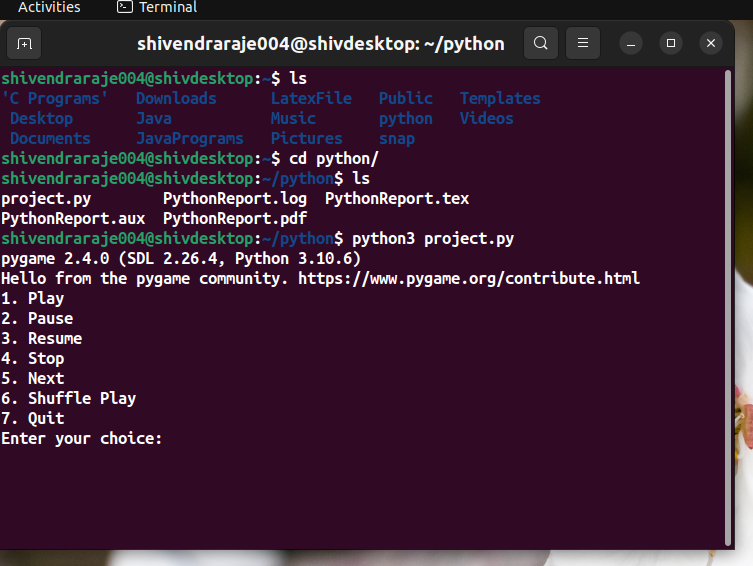
\includegraphics[width=\linewidth]{Interface.png}
		\caption{User Interface}
		\label{Interface}
	\end{figure}
\end{document}





